
\newcommand{\imarrwthree}{2.18in}
\newcommand{\imhspthree}{-0.05in}
\newcommand{\imleftspace}{-0.10in}
\newcommand{\imtextspace}{-0.15in}
\newcommand{\imsinglecol}{2.495in}
\newcommand{\imcaptionspace}{-0.1in}

\newcommand{\insertFigFidelSpace}{
\begin{figure}
\centering
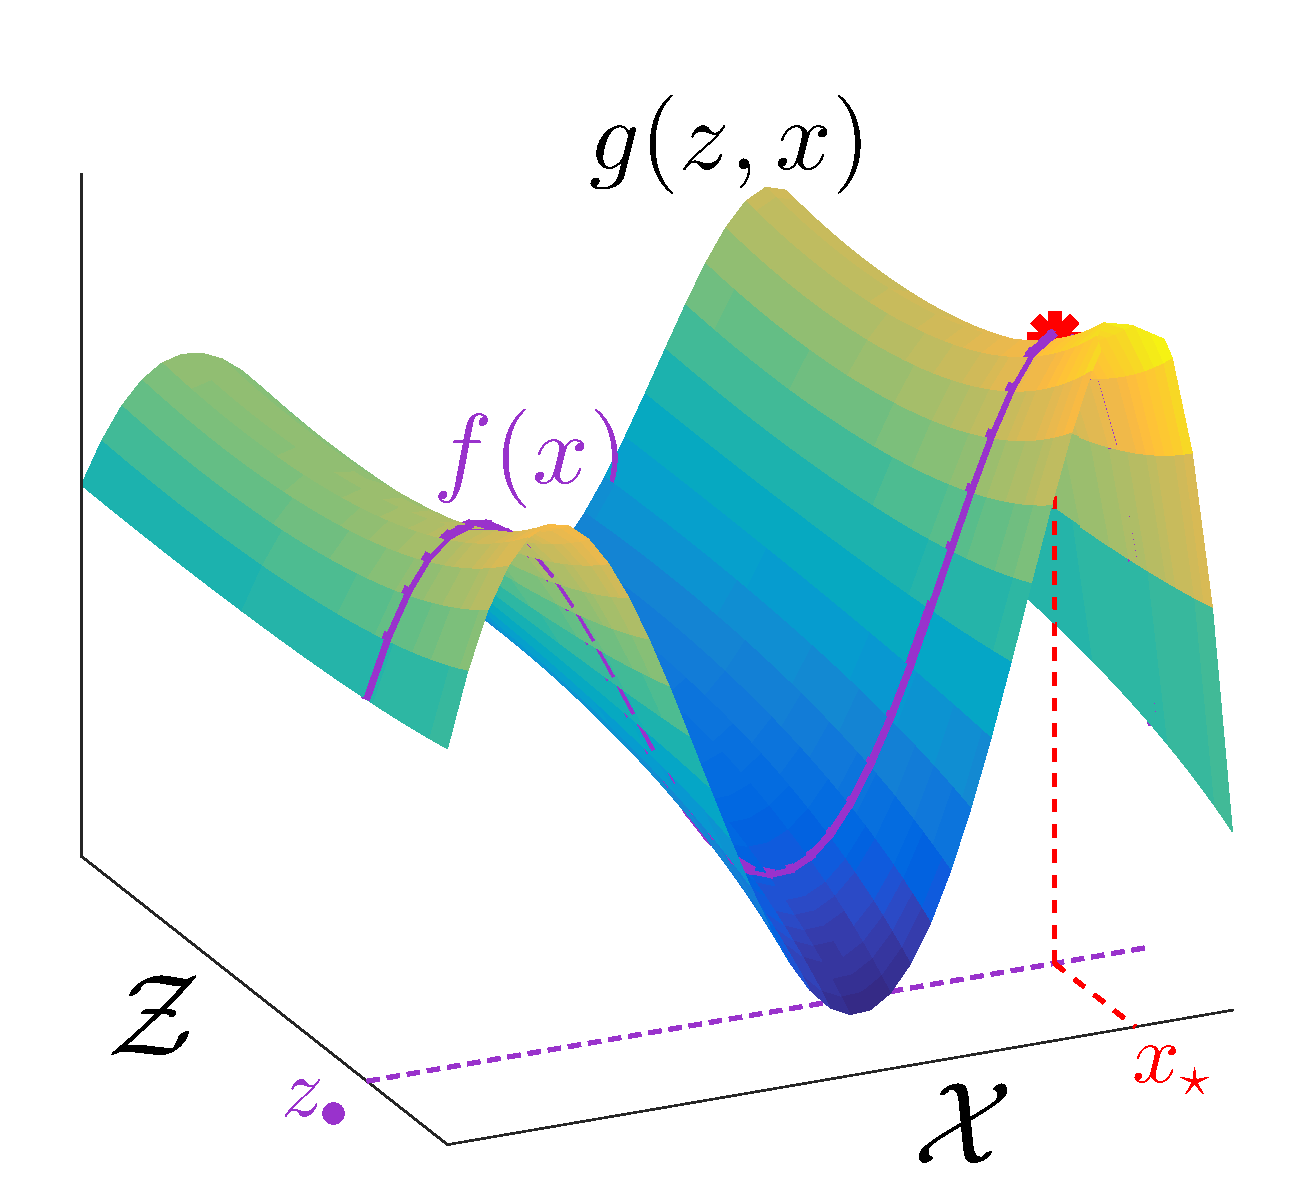
\includegraphics[width=2.2in]{figs/fidel_space}
\vspace{\imcaptionspace}
\caption{\small
\label{fig:fidelSpace}
$g:\Zcal\times\Xcal\rightarrow\RR$ is a function defined on the product space of the
fidelity space $\Zcal$ and domain $\Xcal$.
The purple line is $f(x) = g(\zhf, x)$.
We wish to find the maximiser $\xopt \in \argmax_{x\in\Xcal} f(x)$.
The multi-fidelity framework is attractive when $g$ is smooth across $\Zcal$ as
illustrated in the figure.
\vspace{\imtextspace}
}
\end{figure}
}


\newcommand{\insertFigBWSample}{
\begin{figure}
\centering
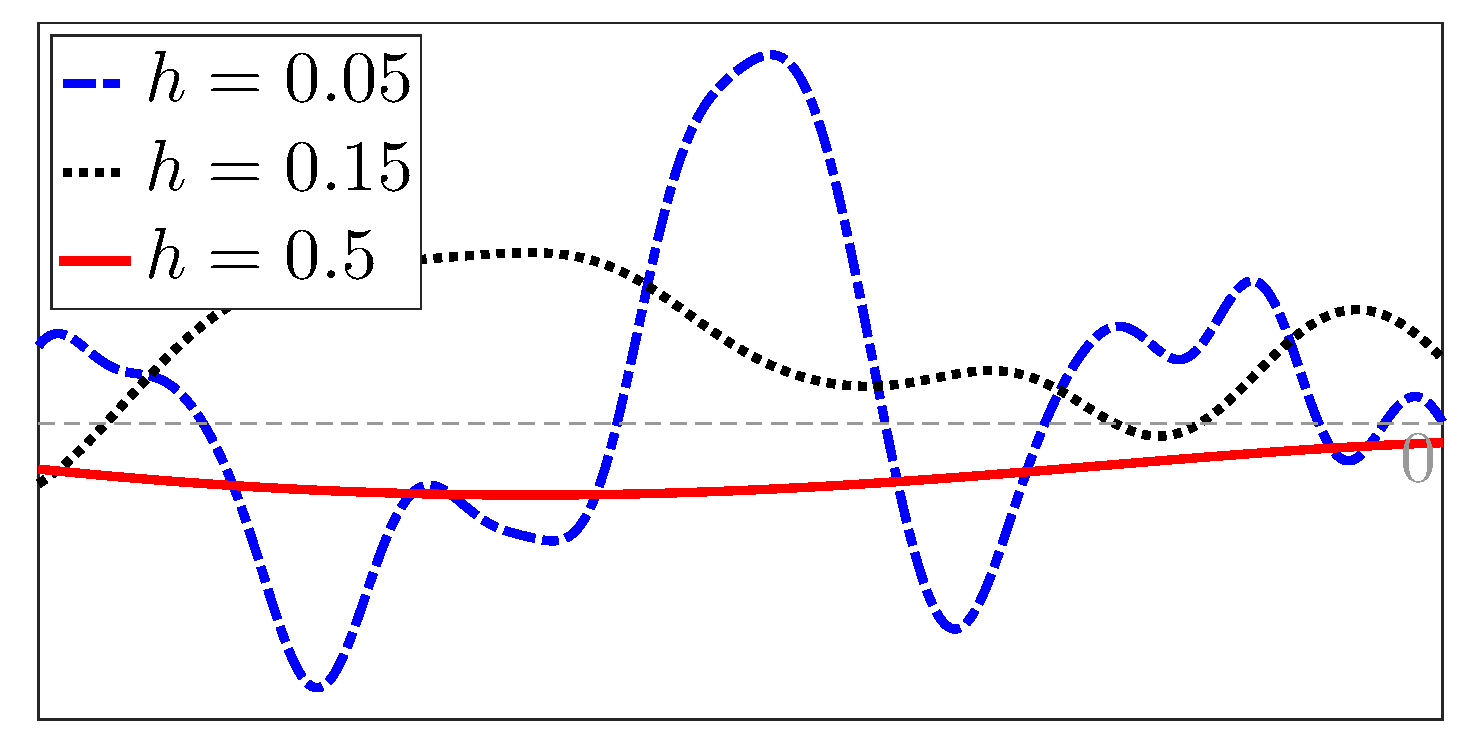
\includegraphics[width=2.0in]{figs/gp_bw_sample}
\vspace{\imcaptionspace}
\caption{\small
\label{fig:gpBWSample}
Samples drawn from a GP with $0$ mean and SE kernel with bandwidths $h=0.01,h=0.15,0.5$.
Samples tend to be smoother across the domain for large bandwidths.
% \vspace{\imtextspace}
\vspace{-0.2in}
}
\end{figure}
}


\newcommand{\insertToyResultsFigure}{
\begin{figure*}
\centering
\hspace{\imleftspace}
\subfigure{
  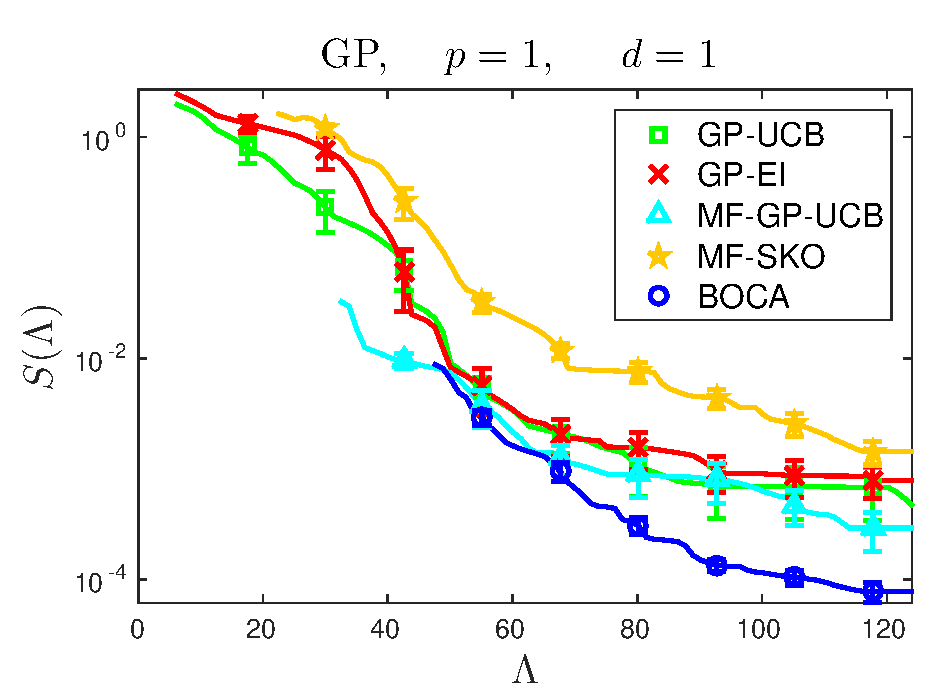
\includegraphics[width=\imarrwthree]{figs/gp} \hspace{\imhspthree}
}
\subfigure{
  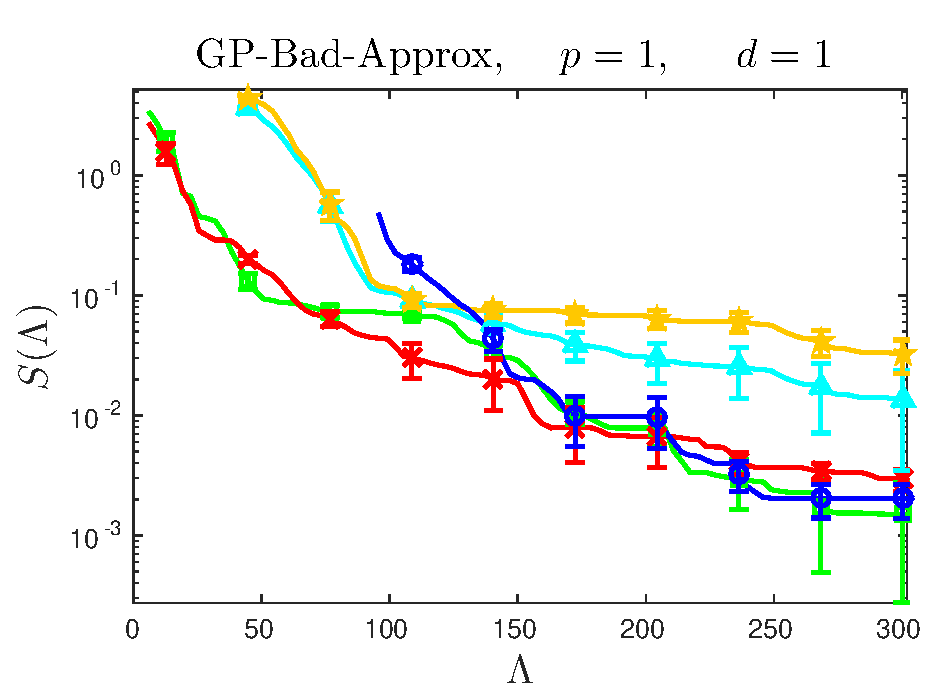
\includegraphics[width=\imarrwthree]{figs/gp_bad} \hspace{\imhspthree}
}
\subfigure{
  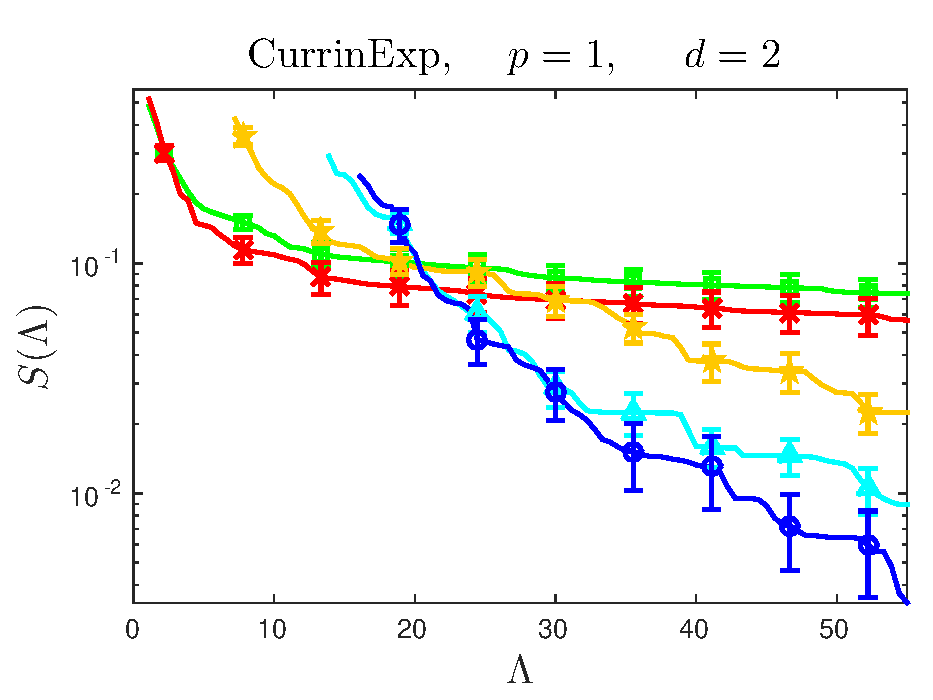
\includegraphics[width=\imarrwthree]{figs/currin_exp} \hspace{\imhspthree}
} \\[\imcaptionspace]
\hspace{\imleftspace}
\subfigure{
  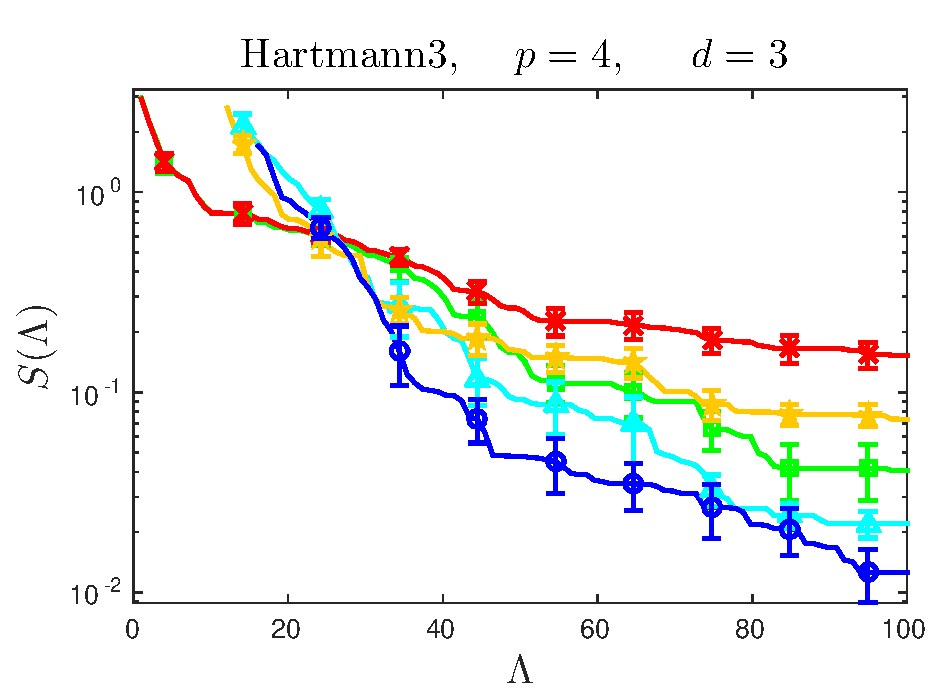
\includegraphics[width=\imarrwthree]{figs/hartmann3} \hspace{\imhspthree}
}
\subfigure{
  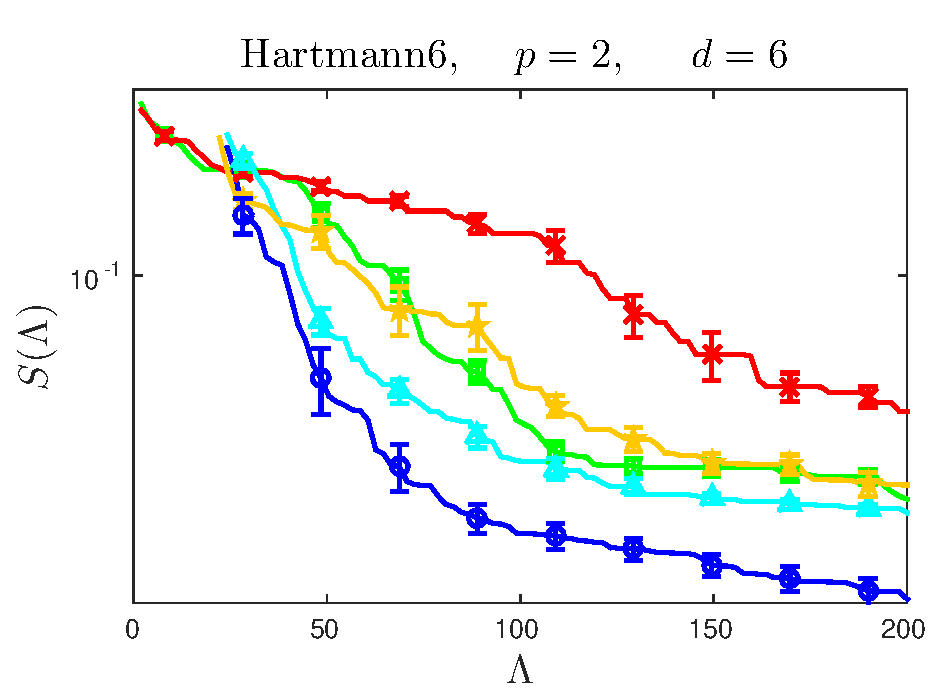
\includegraphics[width=\imarrwthree]{figs/hartmann6} \hspace{\imhspthree}
}
\subfigure{
  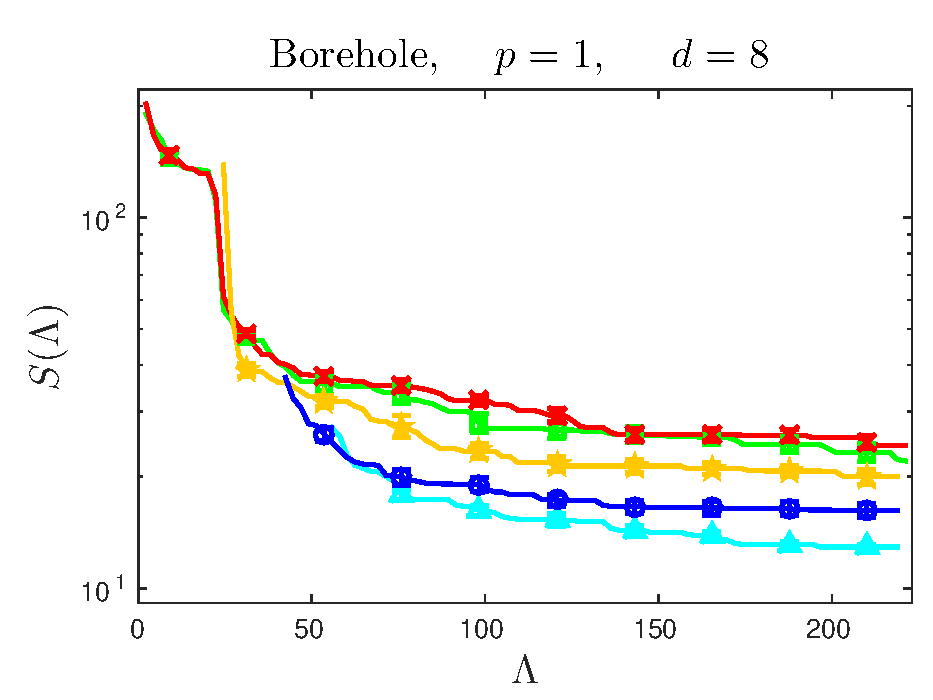
\includegraphics[width=\imarrwthree]{figs/borehole} \hspace{\imhspthree}
% } \\[\imcaptionspace]
} \\[-0.15in]
\caption[]{\small
% The simple regret $S(\capital)$ against capital $\capital$ on $6$ synthetic problems.
Results on $6$ synthetic problems where we plot the simple regret $S(\capital)$ (lower is
better) against the capital $\capital$.
The title states the function used, and the fidelity and domain dimesions.
For the first two figures we used capital $30\cost(\zhf)$, therefore a method which
only queries at $g(\zhf,\cdot)$ can make at most $30$ evaluations.
For the third figure we used $50\cost(\zhf)$, for the fourth $100\cost(\zhf)$ and for
the last $200\cost(\zhf)$ to reflect the dimensionality $d$ of $\Xcal$.
The curves for the multi-fidelity methods start mid-way since they have not queried
at $\zhf$ up until that point.
All curves were produced by averaging over $20$ experiments and the error bars
indicate one standard error.
\vspace{\imtextspace}
\label{fig:toy}
}
\end{figure*}
}




\newcommand{\insertRealResultsFigure}{
\begin{figure*}
\centering
\hspace{\imleftspace}
\subfigure[]{
  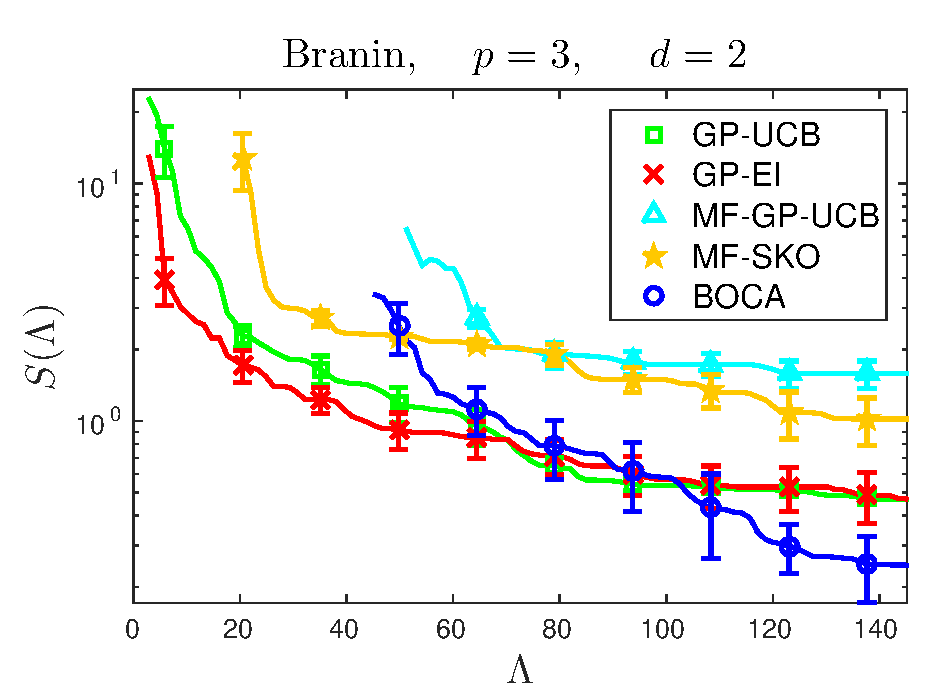
\includegraphics[width=\imarrwthree]{figs/branin} \hspace{\imhspthree}
  \label{fig:branin}
}
\subfigure[]{
  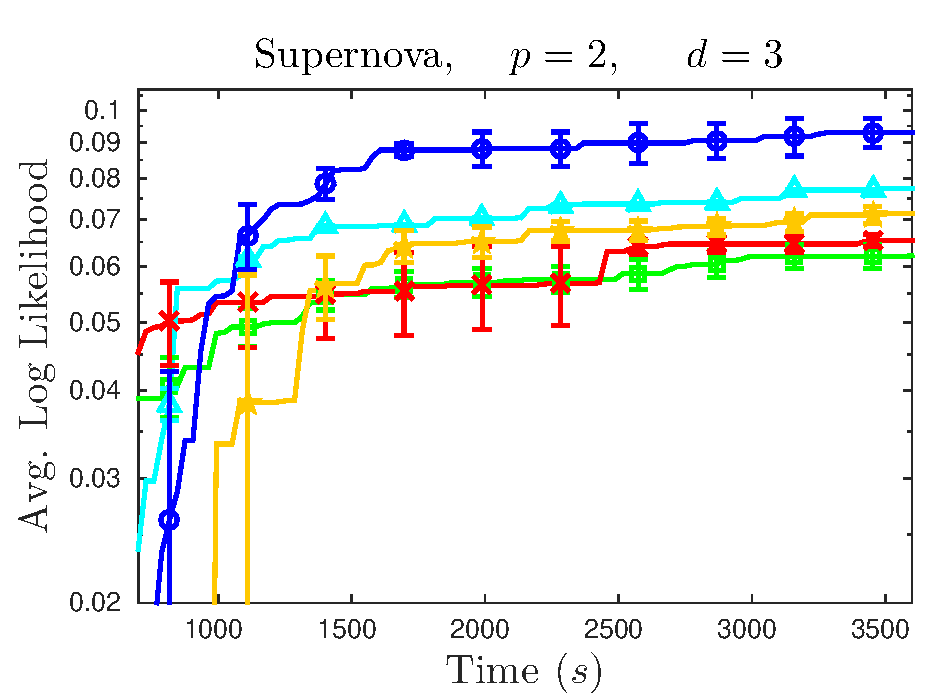
\includegraphics[width=\imarrwthree]{figs/supernova} \hspace{\imhspthree}
  \label{fig:sn}
}
\subfigure[]{
  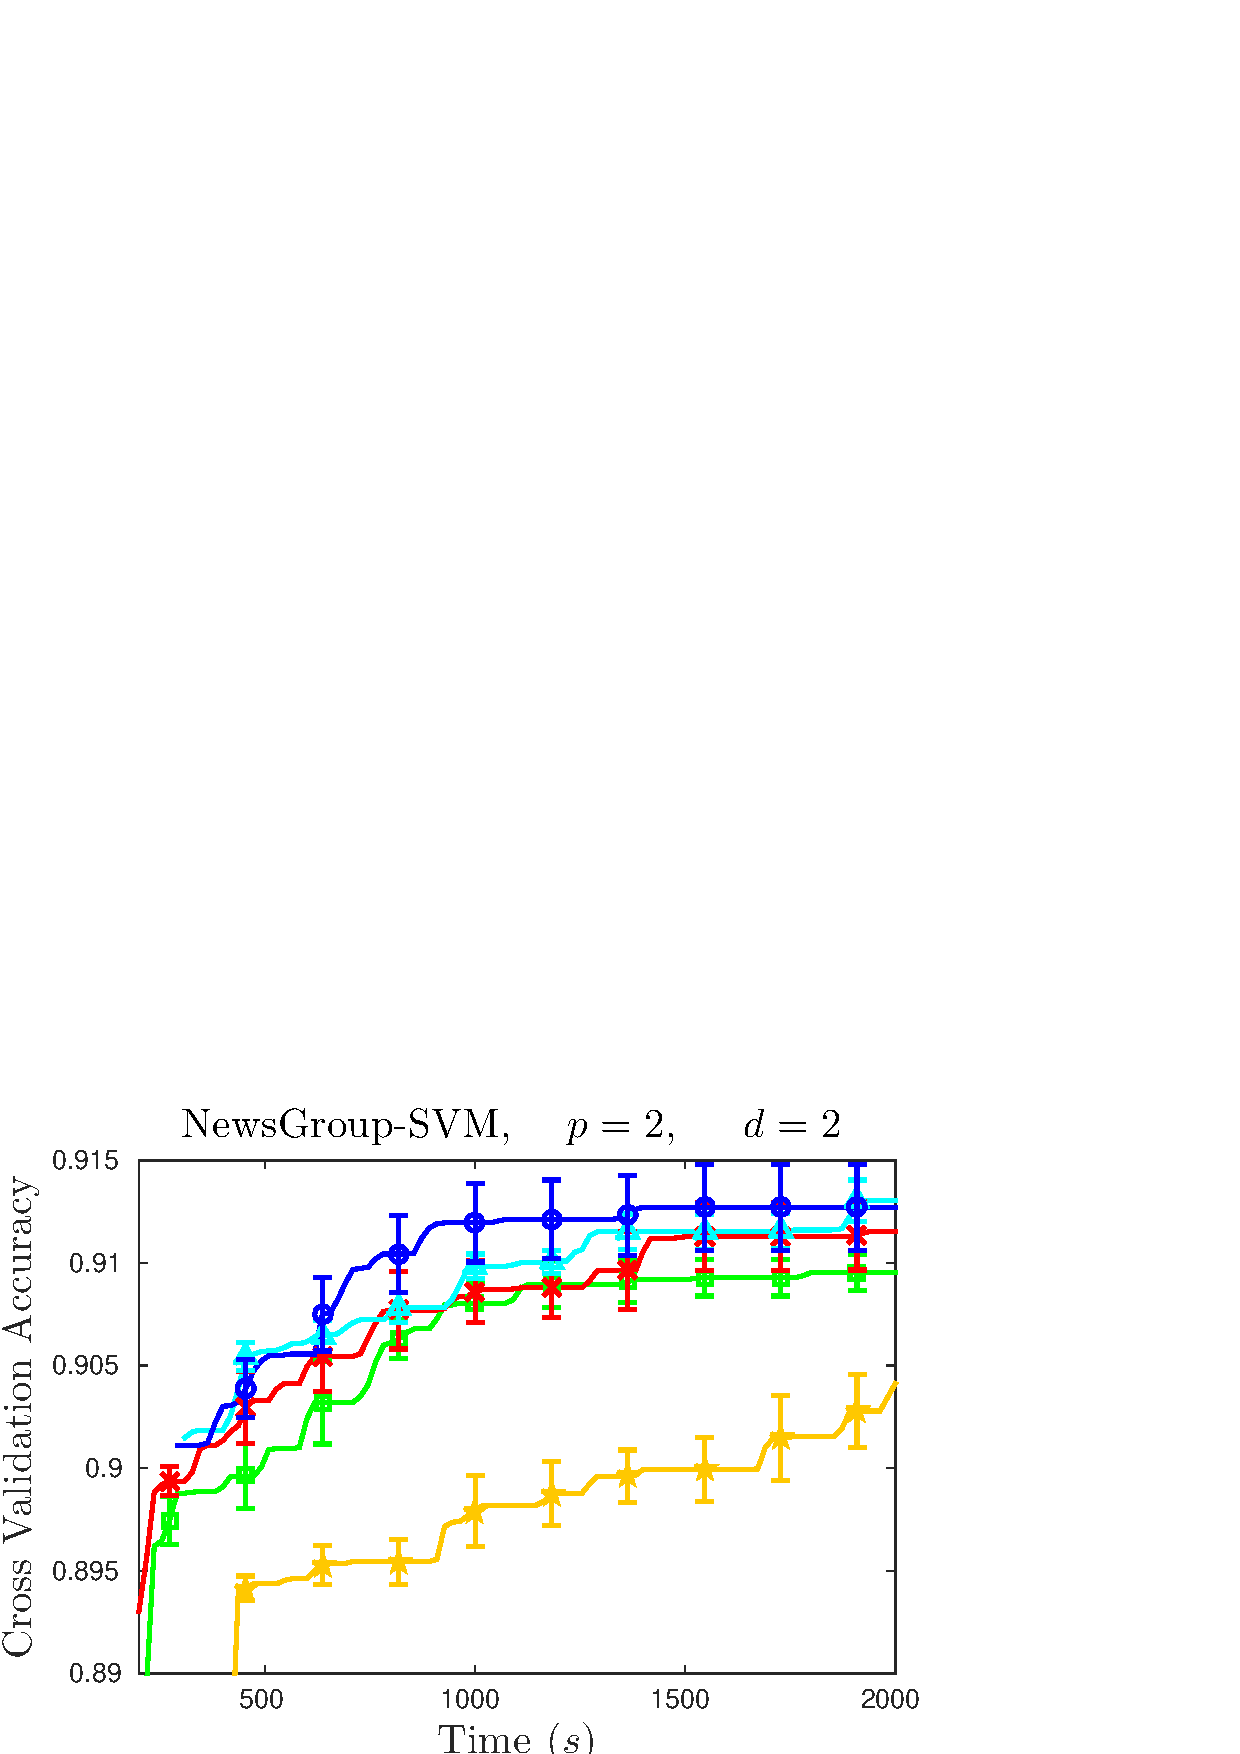
\includegraphics[width=\imarrwthree]{figs/news} \hspace{\imhspthree}
  \label{fig:news}
% } \\[\imcaptionspace]
} \\[-0.15in]
\caption[]{\small
\subref{fig:branin}: The synthetic benchmark with the Branin function where we used a
capital of $50\cost(\zhf)$. See caption under Fig.~\ref{fig:toy} for more details.
\subref{fig:sn},~\subref{fig:news}: Results on the supernova and news group experiments
from sections~\ref{sec:sn} and~\ref{sec:news} respectively. We have plotted the maximum
value (higher is better) against wall clock time.
~\subref{fig:branin} was averaged over $20$ experiments while~\subref{fig:sn}
and~\subref{fig:news} were averaged over $10$ xperiments each.
The error bars indicate one standard error.
\vspace{\imtextspace}
\label{fig:real}
}
\end{figure*}
}
